\section{METHODS}
\label{s:methods}
In the case of a tendon-driven limb with $n$ muscles, the feasible activation space is the unit $n$-hypercube (as muscles can only be activated positively from 0 to a maximal normalized value of 1). As explained in \cite{Valero-Cuevas2009mathematical}, when task constraints are introduced to the system, the feasible activation set is further reduced; in this context, a task is a static force vector produced at the endpoint of the limb, which is represented as a set of inequality and equality constraints. Thus if this simple limb meets all constraints, the feasible activation set is given by the polytope $P$ containing all $a \in \mathbb{R}^n$, that satisfy
\[\textbf{f} = A\textbf{a}, \textbf{a} \in [0,1]^n,\]
where $\textbf{f} \in \mathbb{R}^m$ is a fixed output force vector and $A = J^{-T}RF_o \in \mathbb{R}^{m \times n}$--- where $J$, $R$ and $F_0$ are the matrices of the Jacobian of the limb, the moment arms of the tendons, and the strengths of the muscles, respectively \cite{Valero-Cuevas1998Large,Valero-Cuevas2009mathematical}. 
$P$ is bounded by the unit $n$-cube since all variables $a_i$, $i \in [n]$ are in the interval $[0,1]$. Each constraint of $\textbf{f}= A \textbf{a}$, is a hyperplane in $n-1$ dimensions. If $\textbf{f}$ is a is a feasible submaximal output force and there are no linear depenencies on the constraints, the feasible activation set is a $(n-m)$-dimensional space embedded into the $n$-dimensional unit cube. Note that in our applications, it is safe to assume that no linear dependencies exist.
Consider the following $1 \times 3$ fabricated example, where the task is a 1N unidimensional force. The set of feasible activations is given by the shaded set in Figure \ref{fig:fig_hr}. Since there are three muscles and one constraint the output space is of dimension $3-1 = 2$.
\begin{align*}
&1 = \frac{10}{3}a_1 - \frac{53}{15}a_2 + 2a_3 \\
&a_1, a_2, a_3 \in [0,1],
\end{align*}

\begin{figure}[schematic_arm]
  \label{fig:schematic_arm}
  \centering
  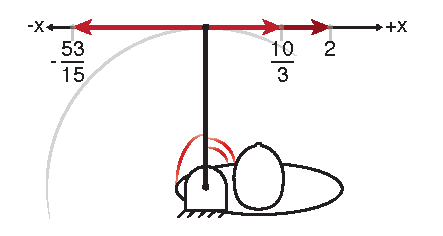
\includegraphics[width=0.5\textwidth]{figs/schematic_arm_1D.pdf}
  \caption{One imagined visualization of the fabricated tendon driven system, with 3 generators.}
  \label{fig:finger}
\end{figure}


\begin{figure}[ht]
  \label{fig:fig_hr}
   \begin{center}
    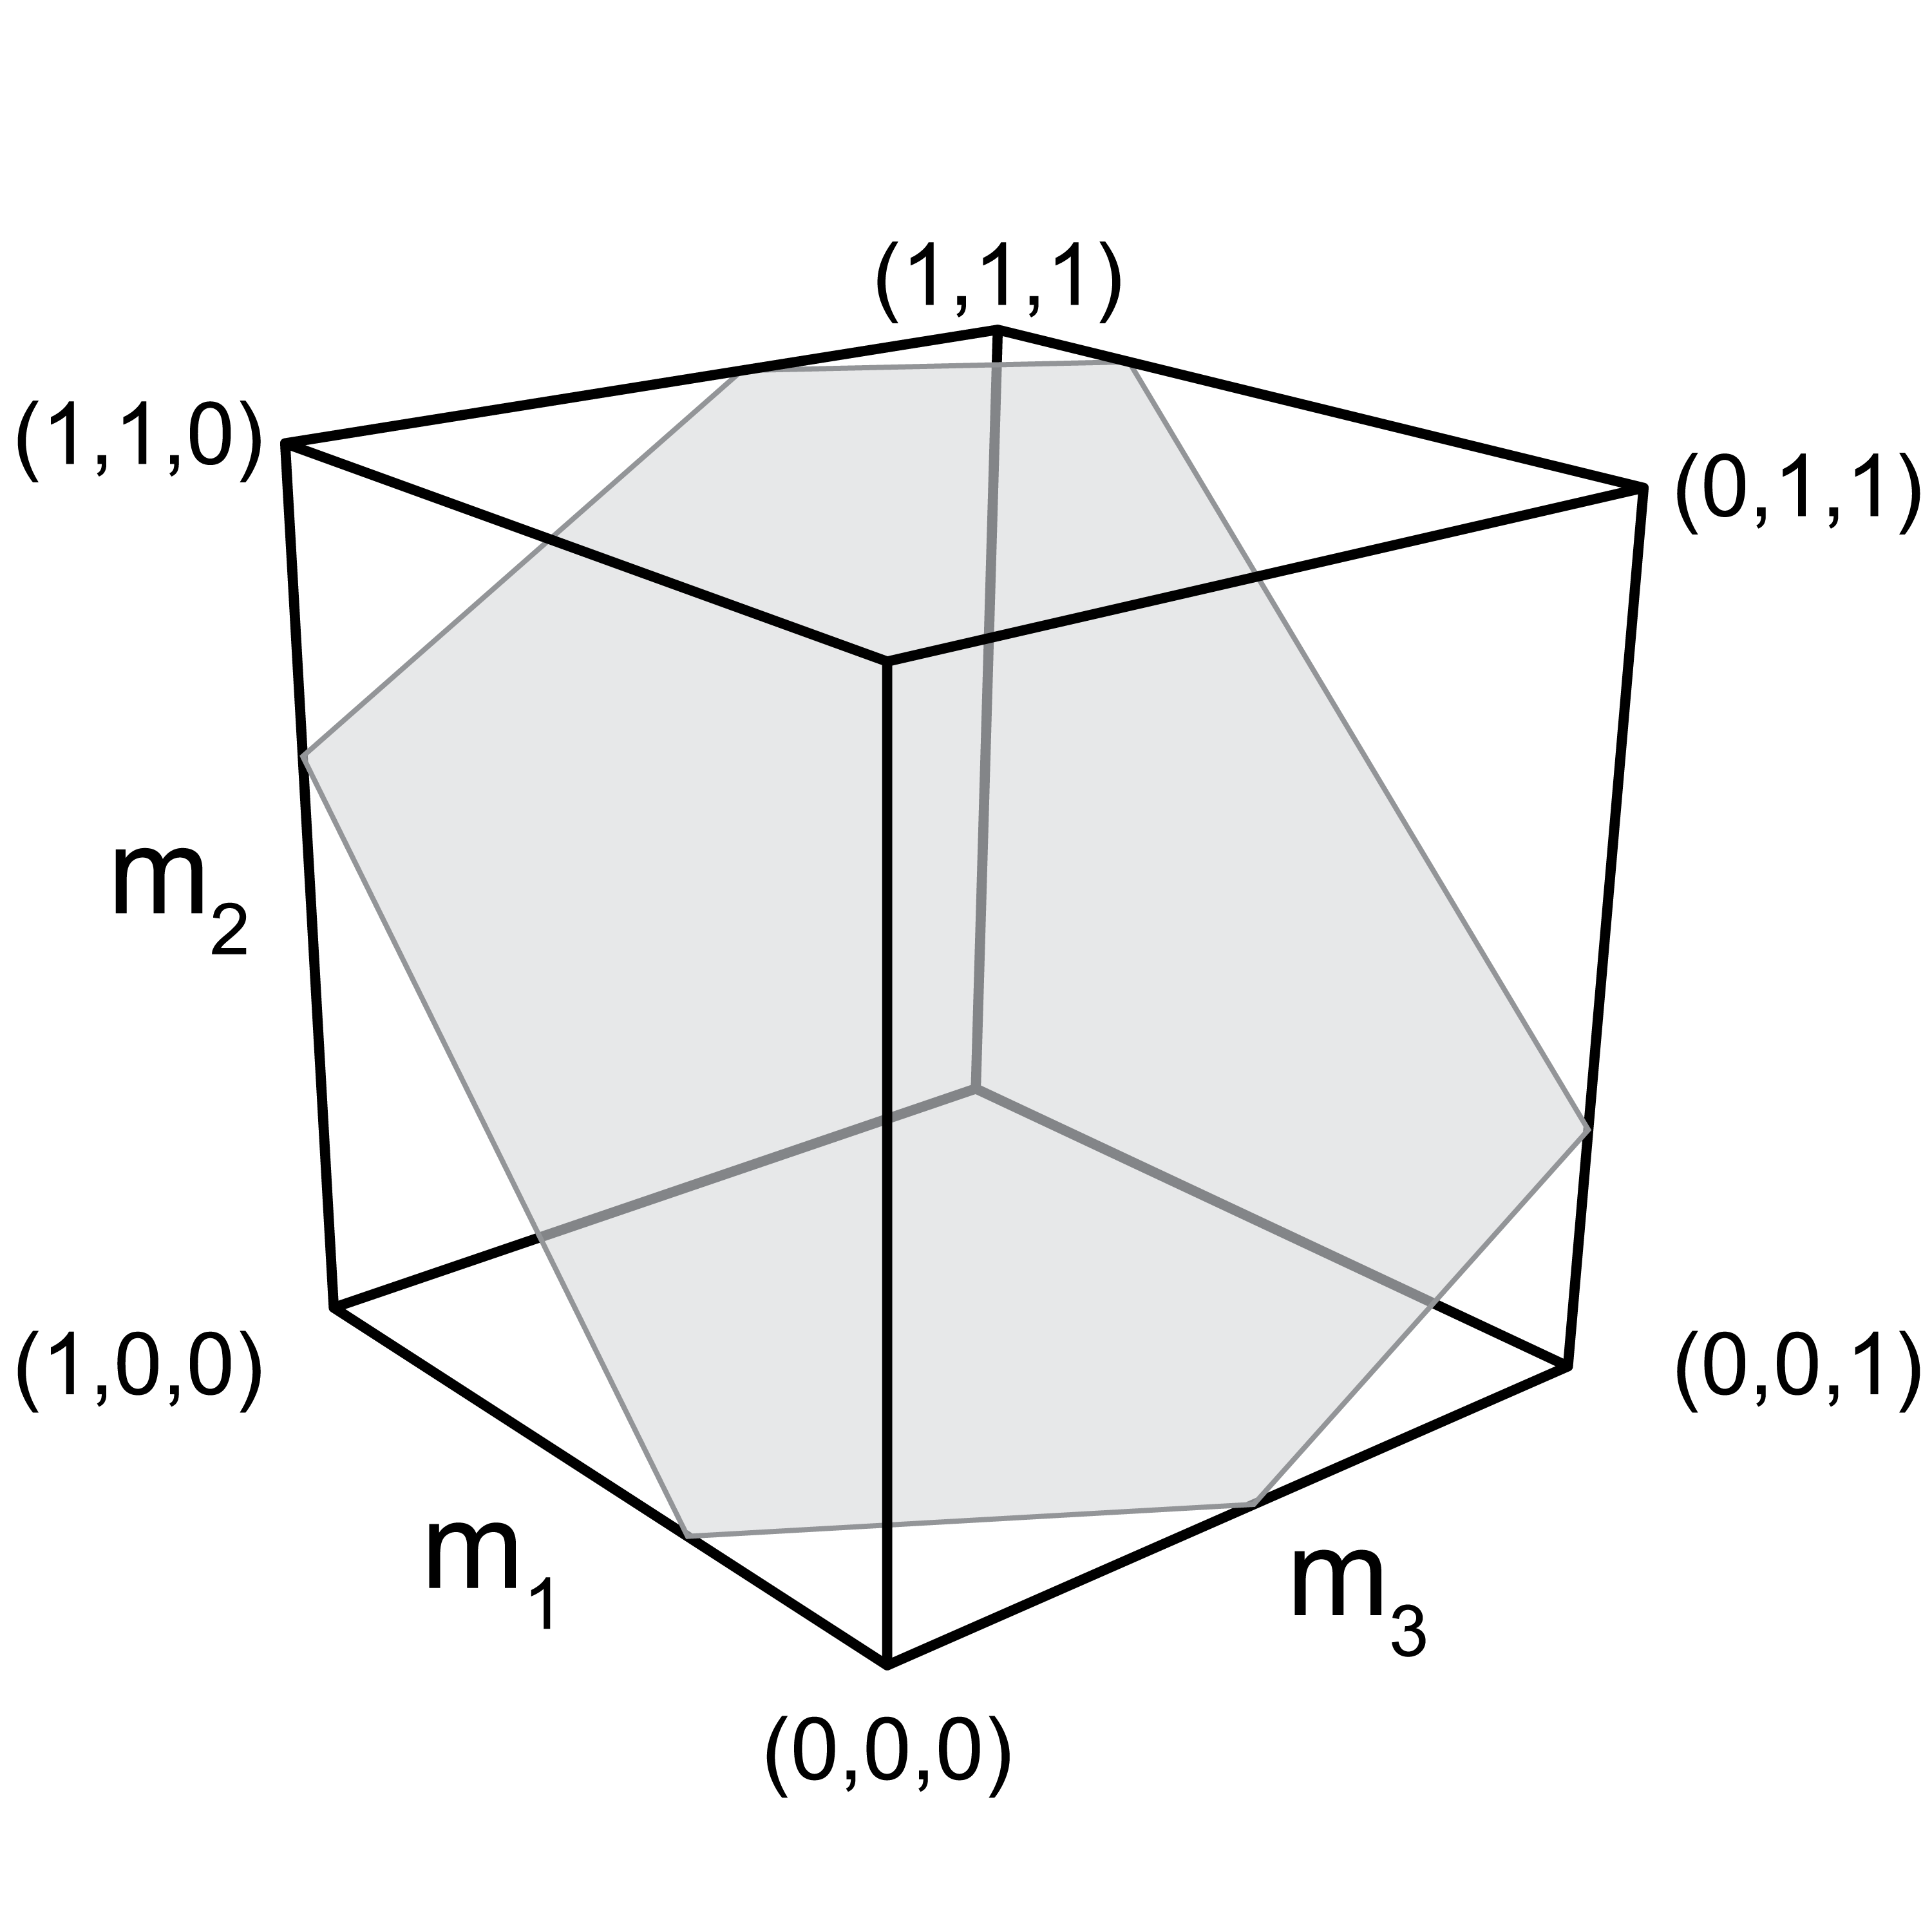
\includegraphics[width=0.25\textwidth]{sections/figs/feasibleactivation.png}
  \end{center}
  \caption{The feasible activation set for a  three-muscle system meeting one functional constraint is a polygon in $\mathbb{R}^3$.} %Note that muscle activations are assumed to be bounded between $0$ and $1$.}
\end{figure}

\subsection{Difficulties of Volume Computation in Higher Dimension}

Exact volume computations for polytopes is known to be $\#P$-hard \cite{Dyer}. Several algorithms have been surveyed and implemented, but can only handle up to 10 dimensions \cite{Bueler2}.  
%We aimed to compare the relative volumes of different sections of the activation space; however, exact volume computations are computationally intractable in dimensions beyond [maytodo cite]. 
Recent muscle system models we have used have been 31 dimensional \cite{Valero-Cuevas2015high-dimensional}, and other muscle models have over 40 muscles involved \cite{arnold2010model, kutch2012challenges, hamner2010muscle, de2014human}, thereby limiting the feasibility of using direct volume computations. Instead, we chose to uniformly sample the continuous space, effectively approximating the shape of the polytope by calculating point densities. %[maytodo mention whether the volume computation is a closed-form solution]

\subsection{Hit-and-Run algorithm}
\label{ss:hitrun}
We chose to sample the activation space with the Hit-and-Run method that is known to converge to the uniform distribution across an< convex body $K$ \cite{smith1984efficient}.
It is a generalization of the discrete Markov chains and recursively samples a sequence of points in $K$ as described below.
The mixing time is known to be $\mathcal{O}^*(n^2R^2/r^2)$, where $r$ and $R$ are the radii of the inscribed and cicumscribed ball of $K$ respectively \cite{Dyer, Lovasz}.
I.e., after $\mathcal{O}^*(n^2R^2/r^2)$ steps, the Hit-and-Run algorithm has sampled a point uniformly at random (u.a.r.) in $K$.
Unfortunately the hidden constant is large, which makes the problem practically almost infeasible.
However experimental results suggest that a number of points linear w.r.t.\ to the dimension suffices; this will be discussed in Section \ref{sec_lengthrun}.
As the feasible activation space of the muscles are given by a convex polytope, this method can be directly applied for our problem.
We chose Hit-and-run because of its easy structure and mixing guarantee; however, it would be interesting to compare Hit-and-Run with the Grid Walk or Ball walk (similar sampling paradigms) \cite{Vempala}.

The Hit-and-Run walk on $P$ is defined as follows (it works analogously for any convex body):
\begin{enumerate}
\item Find a starting point $\textbf{p}$ of $P$. %(Figure \ref{fig:hitruncube}a) .
\item Generate a random direction from $\textbf{p}$ in $P$ (uniformly at random over all directions) (Figure \ref{fig:hitruncube}a).
\item Find the intersection points of the random direction with the boundary of the polytope (Figure \ref{fig:hitruncube}b).
\item Choose a point u.a.r.\ on this line segment given by the intersection points (Figure \ref{fig:hitruncube}c). 
\item Repeat from $2.$ the above steps with the new point as the starting point .
\end{enumerate}

\begin{figure}[h]
\centering
\includegraphics[width=0.5\textwidth,page=10]{sections/figs/HitandRunSchematics_all.pdf}
\caption{Graphical description of the Hit-and-Run algorithm.}
\label{fig:hitruncube}
\end{figure}

\begin{figure}[h]
\centering
\includegraphics[width=0.3\textwidth,page=9]{sections/figs/HitandRunSchematics_all.pdf}
\caption{Uniform distribution aross the feasible activation space.\ In the schematic arm example, the distribution is represented within a 2D plane.}
\label{fig:posthitrun_distribution}
\end{figure}

\subsection{Implementation of Hit-and-Run}
To find a starting point in $P$, the polytope given by
\[\textbf{f} = A\textbf{a}, \textbf{a} \in [0,1]^n,\]
we only need to find a feasible activation vector. For the Hit-and-Run algorithm to mix faster we want the starting point not close to a vertex of the polytope \cite{Lovasz}. %centrally located point within the polytope- that way, the early points will not be clustered in a corner [maytodo cite]. 
We use the following standard trick with slack variables $\epsilon_i$, which for applications often gives a good starting point.% to select a point where activations $a_i$ for all muscles are far from 0 and 1, thereby finding a solution central within $P$ [maytodo cite the use of slack variables to improve mixing time].

\begin{equation}\label{eq:LP_r}
\begin{array}{lrcl}
\mbox{maximize} & \sum_{i=1}^n \epsilon_i \\ 
\mbox{subject to} & \textbf{f} &=& A\textbf{a}\\
  & a_i &\in& [\epsilon_i, 1- \epsilon_i], \hspace{5mm} \forall i \in \{1,\dots,n\}  \\
  & \epsilon_i &\geq& 0, \hspace{5mm} \forall i \in \{1,\dots,n\}.  
\end{array}
\end{equation}


The rest of the implementation of the Hit-and-Run algorithm is straight forward except for the choice of the random direction. How do we sample u.a.r.\ from all directions in $P$? Suppose that $\textbf{q}$ is a direction in $P$ and $\textbf{p} \in P$. Then by definition of $P$, $\textbf{q}$ must satisfy $\textbf{f} = A(\textbf{p}+\textbf{q})$. Since $\textbf{p} \in P$, we know that $\textbf{f} = A\textbf{p}$ and therefore 
\[\textbf{f} = A(\textbf{p} + \textbf{q}) = \textbf{f} + A\textbf{q} \Rightarrow A\textbf{q} = 0. \]

Hence we need to choose directions uniformly at random from all directions in the vectorspace 
\[V = \{\textbf{q} \in \mathbb{R}^n | A\textbf{q} = 0\}.\]

As shown by Marsaglia this can be done as follows \cite{Marsaglia}.
\begin{enumerate}
\item
Find an orthonormal basis $b_1, \dots, b_r \in \mathbb{R}^{n}$ of $A\textbf{q} =0$.
\item
Choose $(\lambda_1, \dots, \lambda_r) \in \mathcal{N}(0,1)^r$ (from the Gaussian distribution).
\item
$\sum_{i=1}^r \lambda_i b_i$ is a u.a.r.\ direction.
\end{enumerate}
A basis of a vectorspace $V$ is a minimal set of vectors that generate $V$, and it is orthonormal if the vectors are pairwise orthogonal (perpendicular) and have unit length. Using basic linear algebra one can find a basis for $\{q \in \mathbb{R}^n | A\textbf{q} = 0\}$ and orthogonalize with the well known Gram-Schmidt method (for details see e.g.\ \cite{Robertson}). Note that in order to get the desired u.a.r.\ sample the basis needs to be orthonormal. For the limb case we can safely assume that the rows of $A$ are linearly independent and hence $r=n-m$.

\subsection{Mixing Time}
\label{sec_lengthrun}
From a given starting point, how many iterations of the Hit-and-Run method are necessary to reach a u.a.r.\ point? For convex polygons in higher dimensions up to $40$, experimental results suggest that $\mathcal{O}(n)$ steps of the Hit-and-Run algorithm are sufficient.
In particular Emiris and Fisikopoulos paper suggest that $(10 + \frac{10}{n})n$ steps are enough to converge upon the uniform distribution \cite{emiris2013efficient}, while in Ge et al.'s paper every point of the Hit-and-Run algorithm is used in the sample \cite{Ge}. 

\subsection{Realistic index finger model}
\label{ss:finger}
We used our published model in \cite{Valero-Cuevas1998Large} to find matrix $A \in \mathbb{R}^{4 \times 7}$, where $\textbf{a} \in \mathbb{R}^7$; the four degrees of freedom were ad-abduction, flexion-extension at the metacarpophalangeal joint, and flexion-extension at the proximal and distal interphalangeal joints.
The force direction we simulated are visible in Figure \ref{fig:finger}.
In this model, for each input we collected 1.000.000 points and sampled every 100th point.
In addition to the Hit-and-Run algorithm we computed the theoretical maximum and minimum activation for each muscle for the given force; the difference between the theoretical and observed bounds for all muscles is smaller than 0.001 (Figures \ref{fig:raw_histograms} and \ref{fig:Z_progression}).

\begin{figure}[htbp]
  \centering
  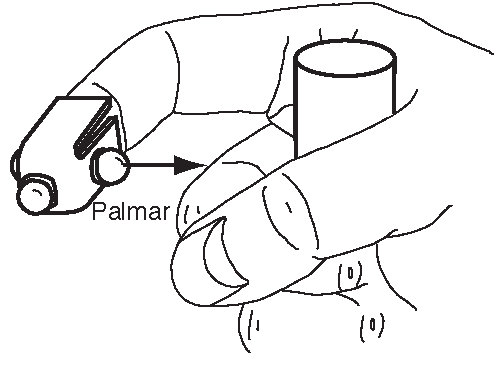
\includegraphics[width=0.5\textwidth]{sections/figs/finger.pdf}
  \caption{The index finger model simulated force production in the palmar direction. Adapted from \cite{Valero-Cuevas1998Large}.}
  \label{fig:finger}
\end{figure}

\subsection{Solution projection histograms}
Figure \ref{fig:raw_histograms} shows the activation distribution of each muscle, when activated with $50\%$ of the maximal activation force. We also show the observed activation upper and lower bounds for each muscle (vertical dotted lines).
In Section \ref{sub:activation_spaces_for_increasing_force} we consider the distributions for different forces into palmar direction.
\begin{figure}[!htbp]
\centering
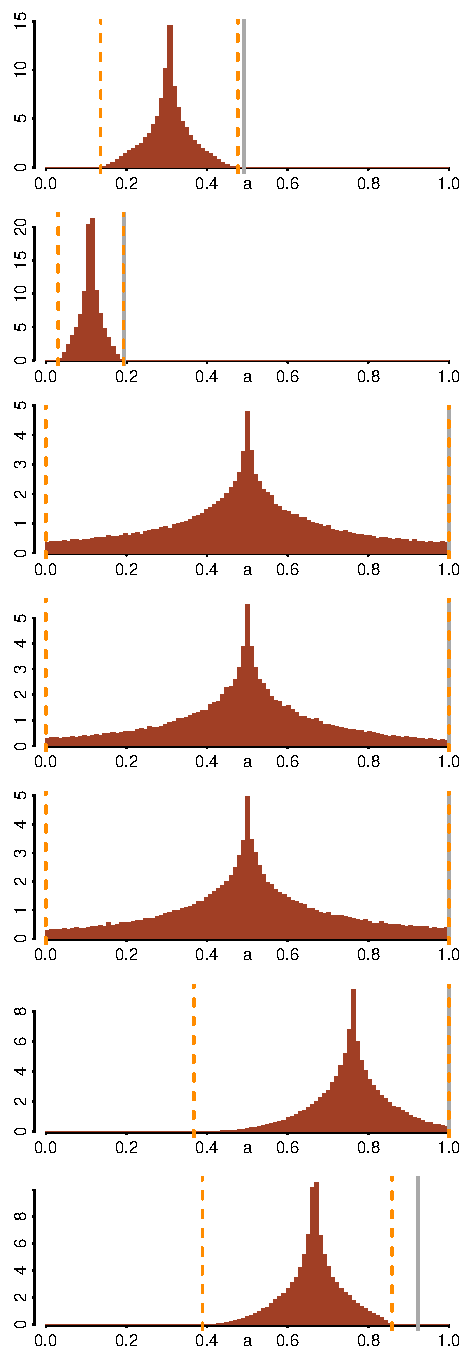
\includegraphics[width=0.5\textwidth]{figs/raw_histograms.pdf}
\caption{Distribution of feasible activations for 50\% of the computed maximal force output in the palmar direction.}
\label{fig:raw_histograms}
\end{figure}

\subsection{Parallel coordinates visualization}
A common way to visualize higher dimensional coordinate data is using parallel coordinates, and has been used in biomechanical studies \ref{bachynskyi2013biomechanical, krekel2010visual}.
To show our sample set of points in the feasible activation space we draw $n$ parallel lines for each of the $n$ muscles.
With the axis labels of the line set between 0 and 1, each point is then represented by connecting their coordinates by $n-1$ lines.
Using an interactive surface we restrict each muscle function to any desired interval- see Figures \ref{fig:parcoord_full} and \ref{fig:parcoords}.
We decided to simulate a 40\% reduction in activation (feasible tendon force production) in three of the muscles innervated by the deep branch of the ulnar nerve- PI, DI, and FDP. 

\subsection{Muscle-metabolic and neural drive cost functions}

For every solution collected, we used popularly-used cost functions: we computed activation $l_1$, $l_2$ and $l_3$ norms, and the tendon-force $l_1^w$, $l_2^w$ and $l_3^w$ weighted norms.


\begin{table}[h]
\centering
\begin{tabular}{@{}ll@{}}
\toprule
\textbf{Name} & \textbf{Cost function}  \\ \midrule
$l_1$            & $\sum_{i=1}^n a_i$                                     \\
$l_2$            & $\sqrt{\sum_{i=1}^n a_i^2}$                                    \\
$l_3$            & $\sqrt[3]{\sum_{i=1}^n a_i^3}$                                   \\
$l_1^w$            & $\sum_{i=1}^n a_i F_{0i}$                                    \\
$l_2^w$            & $\sqrt{\sum_{i=1}^n (a_i F_{0i})^2}$                                  \\
$l_3^w$            & $\sqrt[3]{\sum_{i=1}^n (a_i F_{0i})^3}$                                    \\ \bottomrule
\end{tabular}
\caption{Cost functions and their usage, where $a_i$ and $F_{0i}$ represent a muscle's activation in a given solution and the maximal musculotendon force, respectively.}
\label{cost_function_tabls}
\end{table}

Six additional vertical lines were added to the parallel coordinates plot to represent each cost function. With the same parallel coordinates framework as developed with muscle activation, we can restrict and subset solutions which fall into desired cost-function ranges, thereby masking sub-optimal solutions and highlighting only those meeting the criteria.
For a given point $\textbf{a} \in \mathbb{R}^n$ we are interested in the associated cost of every solution collected through Hit-and-Run.
